\chapter{Simulationsergebnis}


Simulationsparameter:
\begin{itemize}
\item DimX, DimY: 800x800
\item fixed agents: 12
\item fixed agents radius: DimX/6
\item moving agents: 100 000
\item moving agents initial: random position/direction
\item moving agents lookahead radius: 100
\item influence factor: 0,5
\end{itemize}

\begin{figure}[htb]
	\centering
		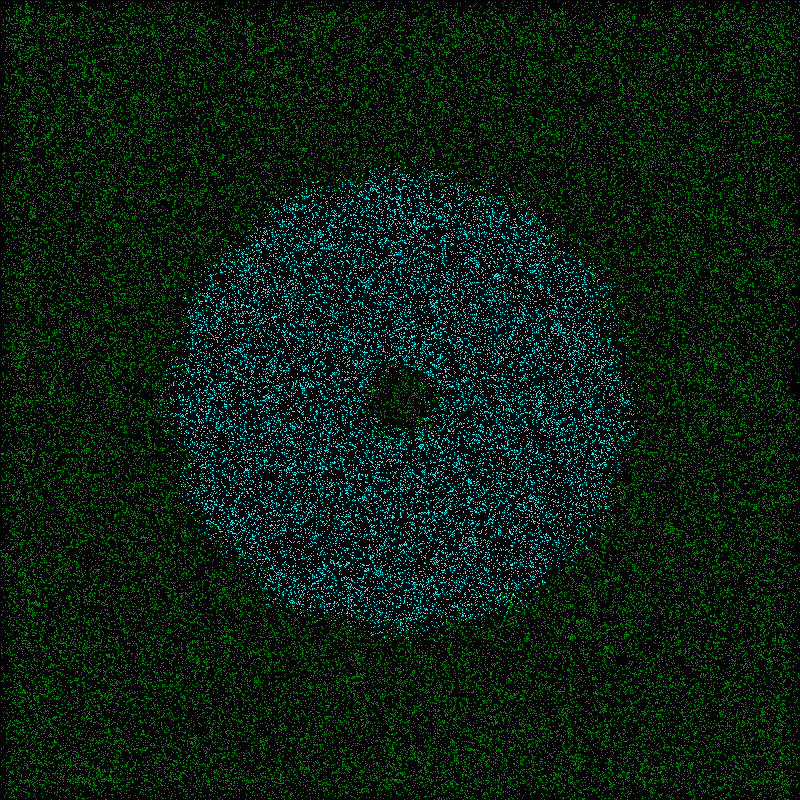
\includegraphics[width=0.9\textwidth,totalheight=0.9\textwidth]{chapter2/plot1_1.png}
	\caption{Sim1, Step 1}
	\label{fig:plot1_1}
\end{figure}

\begin{figure}[htb]
	\centering
		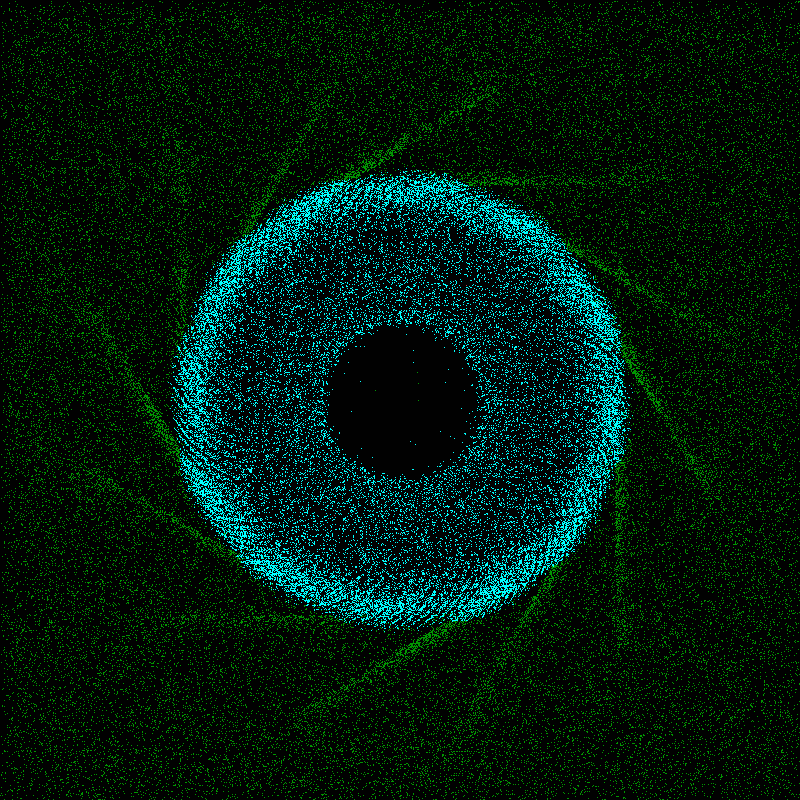
\includegraphics[width=0.9\textwidth,totalheight=0.9\textwidth]{chapter2/plot1_25.png}
	\caption{Sim1, Step 25}
	\label{fig:plot1_25}
\end{figure}

\begin{figure}[htb]
	\centering
		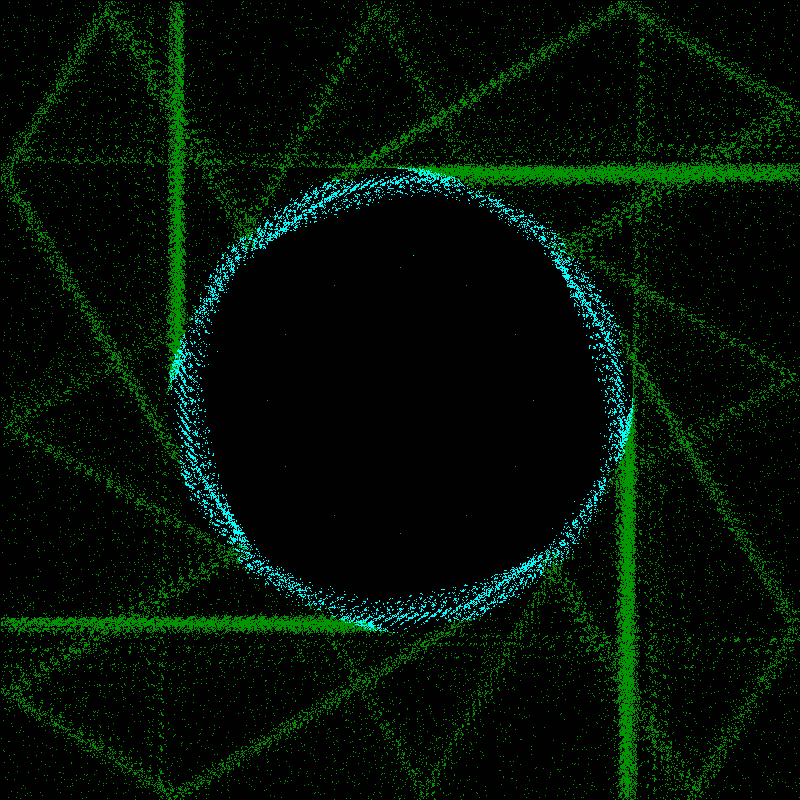
\includegraphics[width=0.9\textwidth,totalheight=0.9\textwidth]{chapter2/plot1_200.png}
	\caption{Sim1, Step200}
	\label{fig:plot1_200}
\end{figure}

\begin{figure}[htb]
	\centering
		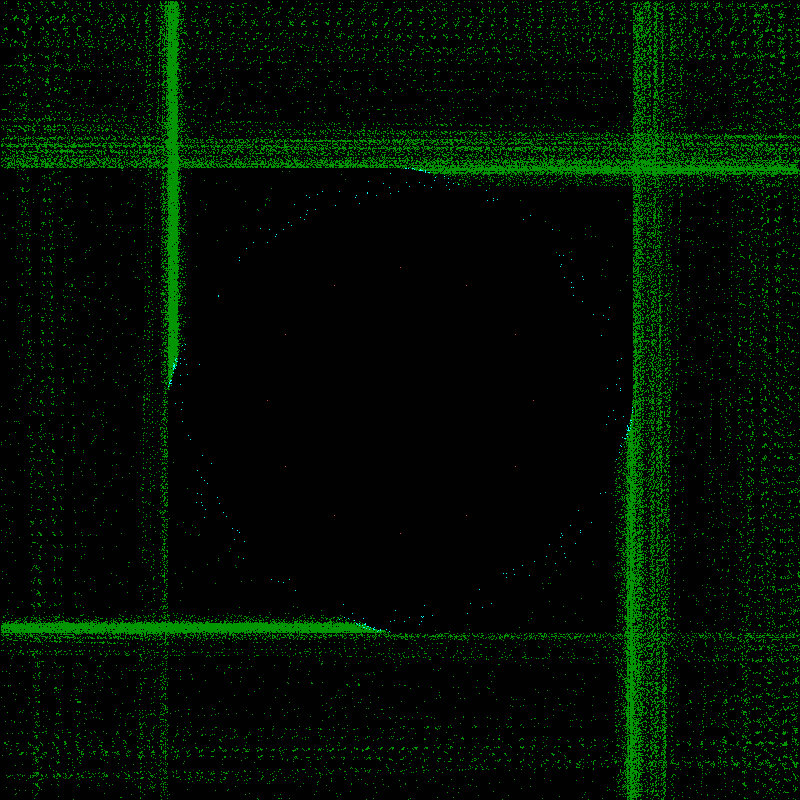
\includegraphics[width=0.9\textwidth,totalheight=0.9\textwidth]{chapter2/plot1_1000.png}
	\caption{Sim1, Step1000}
	\label{fig:plot1_1000}
\end{figure}

In Abbildung \ref{fig:plot1_1} ist die Ausgangssituation dargestellt. Zu sehen ist die zuf�llige Verteilung der beweglichen Agenten. Bewegen sich die Agenten frei, sind diese gr�n eingezeichnet, sind sie von einem fixen Agenten beeinflusst(Parameter ''moving agents lookahead radius``) sind sie t�rkis eingezeichnet. Fixe Agenten, welche die Bewegungsrichtung vorgeben, sind rot eingezeichnet. In diesem Anfangszustand mit vielen Agenten sind diese kaum erkennbar, da sie in der Zeichenebene unter den beweglichen Agenten liegen.\newline

\vspace{0.4cm}

Wie man an Abbildung \ref{fig:plot1_25} und \ref{fig:plot1_200} beobachten kann, finden sich alle beweglichen Agenten nach einer endlichen Zeit in einem Orbit um die fixen Agenten ein. Wie wir aus der Aufgabenstellung wissen, besitzen alle fixen Agenten eine Wegweiser-Vektor der normal auf dem Eigenvektor vom Mittelpunkt des Kreises steht. D.h. dass sich alle beweglichen Agenten folglich in endlicher Zeit auf den �ussersten Radius zubewegen m�ssen und diesen auch folglich irgendwann verlassen m�ssen. In Abbildung \ref{fig:plot1_200} ist gut zu erkennen wie s�mtliche beweglichen Agenten regelm��ig den ''Orbit`` verlassen um an der Aussenwand des Simulationsfeldes wieder abzuprallen. Dieses Abprallen steht so nciht in der Aufgabenstellung, und wurde von uns sinnvollerweise hinzugef�gt. Ohne dieses vorgegebene Verhalten ist zu erwarten, dass sich gegen unendlichen Simulationsverlauf alle Agenten  unendlich weit entfernen.\newline

\vspace{0.4cm}

Eine interessante Beobachtung ist auch, dass sich die Austrittspunkte aus dem Orbit immer kurz vor dem Einfluss eines im Orbit folgendem fixen Agenten befinden. Diese Beobachtung l�sst sich auch mit dem im letzten Punkt behandelten Verhalten erkl�ren, dass sich alle beweglichen Agenten immer weiter richtung �ussersten Orbit bewegen und auch am ehesten den rbit verlassen wenn die Anzahl der beinflussenden fixen Agenten am geringsten ist. Weiters ist mit fortlaufender Simulation zu beobachten dass besonders bei den in N,O,S,W stehenden fixen Agenten die beweglichen Agenten austreten bzw. h�ufen. Das ist dadurch zu erkl�ren, dass bei einer Ber�hrung der imagin�ren Wand die Agenten zur�ckgeworfen werden mit einer einfachen invertierung der kollidierenden Bewegungsrichtung. Vergleichbar auch mit einem Abprall einer Billardkugel an einer Bande. Da nun bei einem Austritt in N,O,S,W die Agenten sich auf einem fast direktem Kollisionskurs mit der begrenzenden Wand befinden, werden diese bei Erreichen auch fast direkt zur�ckgeworfen. Damit komme selbige wieder direkt in den Einfluss des gleichen fixen Agenten was in Folge wieder eine Ablenkung in die gegengesetzte Richtung gegen Wand bedeutet. Dieses Verhalten wiederholt sich bis sich der Agent im Einfluss eines anderen fixen Agenten(meistens der in Folgerichtung des Orbits) befindet, und von diesem mitabgelenkt wird. Abbildung \ref{fig:plot1_1000} best�tigt diese Theorie.